% !TEX TS-program = pdflatex
% !TEX encoding = UTF-8 Unicode
%
% -----------------------------------------------------
% LaTeX-Vorlage
%
% LABREPORT v1
% von Markus Kn�sel frei nach KOMA-Script-Klassen
% -----------------------------------------------------
%
\documentclass[11pt,titlepage]{scrartcl}		% Schriftgr��e festlegen, standard 10pt 
%
\usepackage[latin1]{inputenc}				% input encoding f�r vim/utf8/Umlaute
\usepackage[T1]{fontenc}
\usepackage{lmodern} 
%
% -----------------------------------------------------
\usepackage{geometry} 					% legt die Blattgr��e und Randabst�nde fest
\geometry{a4paper}
\geometry{margin=3cm,top=2.5cm,bottom=2.5cm}
%
%
%
%
%
%
% -----------------------------------------------------
\usepackage{graphicx} 					% support the \includegraphics command and options
\usepackage[parfill]{parskip}				% Activate to begin paragraphs with an empty line rather than an indent
\usepackage{booktabs}					% for much better looking tables
%\usepackage{array}					% for better arrays (eg matrices) in maths
\usepackage{paralist}					% very flexible & customisable lists (eg. enumerate/itemize, etc.)
\usepackage{verbatim}					% adds environment for commenting out blocks of text & for better verbatim
\usepackage{subfig}					% make it possible to include more than one captioned figure/table in a single float
\usepackage{color}
\usepackage[german]{babel}
\usepackage{units}
\usepackage[onehalfspacing]{setspace}
\usepackage{amsmath,amsfonts,amssymb}
\usepackage{icomma,units}
\usepackage{enumerate}
\usepackage[margin=10pt,font=small,labelfont=bf,labelsep=endash]{caption}
\usepackage{chemmacros}
\usepackage{chemfig}
\usepackage{PSTricks}
\usepackage{epstopdf}
\usepackage[ngerman=ngerman-x-latest]{hyphsubst}
\usepackage{pgfplots}
\usepackage{pgfplotstable}
%
%
%
%
% ---------- HEADERS & FOOTERS ------------------------
\usepackage{fancyhdr} % This should be set AFTER setting up the page geometry
\pagestyle{fancy} % options: empty , plain , fancy
%\renewcommand{\headrulewidth}{0pt} % customise the layout...
\lhead{Markus Kn�sel}\chead{}\rhead{\textsc{Physikalische Chemie II}}
%\lfoot{}\cfoot{\thepage}\rfoot{}
%
%
%
%
% ---------- SECTION TITLE APPEARANCE -----------------
\usepackage{sectsty}
\definecolor{cyan}{RGB}{30,103,182}      % hellgruener Rahmen
\allsectionsfont{\mdseries\upshape\textcolor{cyan}} % (See the fntguide.pdf for font help)
%
%
%
%
% ---------- ToC (table of contents) APPEARANCE -------
\usepackage[nottoc,notlof,notlot]{tocbibind} % Put the bibliography in the ToC
\usepackage[titles,subfigure]{tocloft} % Alter the style of the Table of Contents
% \renewcommand{\cftsecfont}{\rmfamily\mdseries\upshape}
% \renewcommand{\cftsecpagefont}{\rmfamily\mdseries\upshape} % No bold!
%
%
%
%
% ---------- TITLEPAGE DETAILS ------------------------
\addtokomafont{subject}{\sc}
\setkomafont{title}{\normalfont}
	\subject{Das Daniell-Element}
	\title{Versuchsprotokoll}
	\subtitle{3812 - Praktikum Physikalische Chemie II}
	\author{\normalfont Markus Kn�sel \\ Matrikelnr. 23 94 86 }
	\date{durchgef�hrt am 30.11.14} % Activate to display a given date or no date (if empty),
\publishers{\normalsize \includegraphics[width=4cm]{unilogo} \\ Fachbereich IV \\ Abteilung f�r Chemie}
%
%
%
%
% ---------- DOCUMENT ---------------------------------
%
\newtagform{equation}{\{}{\}}
\usetagform{equation}
\begin{document}
	\maketitle
	\tableofcontents
	\newpage
%
% ------ Equation/Reaction Counter ---------
\RenewEnviron{reaction}{\begin{equation} \expandafter \ch\expandafter {\BODY} \end{equation}}
\RenewEnviron{reaction*}{\begin{equation*}\expandafter \ch\expandafter{\BODY}\end{equation*}}
\RenewEnviron{reactions}{\begin{align}\expandafter\ch\expandafter{\BODY}\end{align}}
\RenewEnviron{reactions*}{\begin{align*}\expandafter\ch\expandafter{\BODY}\end{align*}}

%	
%
%
%% \section*{\abstractname}
%% Blabla
%
\section{Theoretische Grundlagen}
In diesem Versuch soll das Funktionsprinzip des \emph{Daniell-Elements} verdeutlicht werden. Diese galvanische Zelle wurde 1836 von J. F. Daniell entwickelt und nach ihm benannt. 
%
\subsection{Das Daniell-Element}
\begin{figure}[h]
	\centering
	\scalebox{0.5}{\includegraphics{daniell}}
	\caption{Daniell-Element \textsc{(Ayrton, S. 210)}}
	\label{fig:daniell}
\end{figure}
\begin{quotation}
\textit{The Daniell's Cell consists
of a copper plate c. (\dots), dipping into a solution of
copper sulphate contained in a glass, or glazed, highly
vitrified stoneware jar, J, and a zinc plate, or rod, z, to
which a copper wire, or strip, w, is soldered, dipping into
either dilute sulphuric acid or a solution of zinc sulphate,
the two solutions being separated by a porous partition P,
made of unglazed earthenware, and called a
"`porous pot."' 
The E. M. F. of a Daniell's cell, and of all its
modifications, is roughly 1.1 volts, but it varies from
about 1.07 volts to 1.14 volts, depending on the densities
of the solutions of copper and zinc sulphate. With equidense solutions, and with plates of pure zinc and copper,
the E. M. F. is 1.104 volts. This value is increased by
increasing the density of the copper sulphate solution,
and diminished by increasing the density of the zinc
sulphate solution, and is scarcely at all affected by the
ordinary atmospheric changes of temperature. (\dots) } (\textsc{Ayrton, S.210-211})
\end{quotation}
%
\subsection{Die elektromotorische Kraft}
Erstellt man aus 2 Halbzellen mit unterschiedlichen Standardpotentialen ein galvanisches Element, so entsteht eine Potentialdifferenz. Diese Spannung wird elektromotorische Kraft (EMK) genannt. Aufgrund der auftretenden EMK kann das galvanische Element nun elektrische Arbeit verrichten. In den beiden Halbzellen des Daniell-Elements laufen folgende Reaktionen ab:
\begin{reactions}
	Zn -> Zn^{2+} + 2 \el \\
	Cu^{2+} + 2 \el -> Cu
\end{reactions}
Als Gesamtreaktion ergibt sich:
\begin{reaction}
%	\vspace{14mm}}
	"\OX{o1,\ox{+2,Cu}}\pch[2]"  + "\OX{r1,\ox{0,Zn}}"
	->
	"\OX{o2,\ox{0,Cu}}"  + "\OX{r2,\ox{+2,Zn}}\pch[2]"
\end{reaction}
%\redox(o1,o2)[draw=red,->][3.33]{\small OX: $- 2\el$}
%\redox(r1,r2)[draw=blue,->]{\small RED: $+ 2\el$}
An der Kathode findet die Reduktion statt, an der Anode die Oxidation. Die Anode ist also bei einem galvanischen Element als Minus-Pol (Elektronen�berschu�) zu sehen. Zu beachten ist die Tatsache, da� f�r ein Elektronenflu� durch einen Verbraucher (der an die beiden Elektroden des galvanischen Elements angeschlossen ist) ebenfalls Ladungsaustausch innerhalb des Elements stattfinden mu�. Bei dem Daniell-Element geschieht dies durch \ch{SO4^{2-}}-Ionen, die durch die Wand der Tonzelle hindurchdiffundieren.
%
\begin{figure}[h]
	\centering
	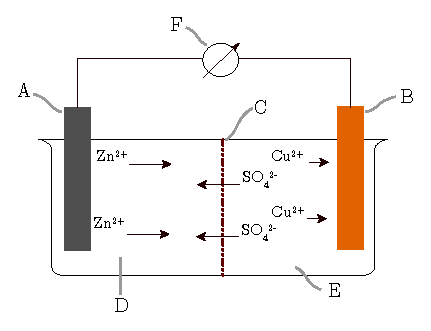
\includegraphics{schema.eps}
	\caption{schematischer Aufbau eines Daniell-Elements mit Zinkelektrode (A), Kupferelektrode (B), por�ser Trennwand (C), Zinksulfatl�sung (D), Kupfersulfatl�sung (E) und Voltmeter (F) (\textsc{Riedel}, S. 348)}
	\label{fig:schema}
\end{figure}
%
%
\section{Versuchsdurchf�hrung}
%
\begin{figure}[h]
	\centering
	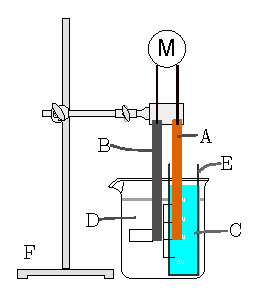
\includegraphics{aufbau.eps}
	\caption{Versuchsaufbau mit Kupferblech (A), Zinkblech (B), \ch{CuSO4}-L�sung (C), \ch{ZnSO4}-L�sung (D), Tonzelle (E) und Stativ mit Klemmen und Elektrodenhalter (F)}
	\label{fig:aufbau}
\end{figure}
\begin{singlespace}
	\small\underline{Ger�te:}~Tonzelle, Becherglas 250~ml, Multimeter, Verbindungskabel, Zinkblech, Kupferblech, 2 Krokodilklemmen, Kleinelektromotor\\[1ex]
	\underline{Chemikalien:}~\ch{CuSO4}-L�sung (1 \unitfrac{mol}{l}), \ch{ZnSO4}-L�sung (1 \unitfrac{mol}{l})\\[1ex]
\end{singlespace}
%
Die Apparatur wird gem�� Abbildung \ref{fig:aufbau} aufgebaut; die Elektroden wurden gewogen. Zu Beginn wird die Spannung des galvanischen Elements mit Hilfe des Multimeters gemessen. Dann wird es durch einen Kleinelektromotor ersetzt und ca. 5 min betrieben. Anschlie�end wird der Stromflu� unterbrochen, die beiden Elektroden vorsichtig mit demineralisiertem Wasser gesp�lt, getrocknet und gewogen.
%
\section{Auswertung}
Die Stoffmenge, die an einer Elektrode w�hrend der Elektrolyse abgeschieden wird oder in L�sung geht, ist proportional zur elektrischen Ladung, die den Elektrolyten durchflie�t. (1. Faraday'sches Gesetz). Folglich kann durch die Auswaage der Elektroden vor und nach der Versuchsdurchf�hrung die insgesamt geflossene Ladungsmenge berechnet werden nach:
\begin{align}
	Q &= n \cdot z \cdot F\\
	&= \frac{m}{M} \cdot z \cdot F
\end{align}
Hierbei ist $n$ die umgesetzte Stoffmenge, $z$ die Anzahl Ladungstr�ger pro Reaktionsschritt, $F$ die Faraday-Konstante. Mit den in Tabelle \ref{tab:gewicht} festgehaltenen Messwerten f�r die umgesetzte Menge ergibt sich f�r die ca. 5 min Betrieb der Zelle ein Ladungsumsatz von:
\begin{align}
	Q &= \frac{0,0019~\si{\gram}}{63,546~\si{\MolMass}} \cdot 2 \cdot 96485~\si{\coulomb\per\mole}\\
	&=5,770~\si{\coulomb} \phantom{\frac{}{}}
\end{align}
Die entspricht bei einer Betriebszeit von 5 min. einem durchschnittlich geflossenem elektrischen Strom von:
\begin{equation}
I = \SI{19}{\milli\ampere}
\end{equation}
%
%
\newpage
\section{Anhang}
%
\begin{table}[h]
	\centering
	\begin{tabular}{l r r}
		\toprule
			 & $m_{Zinkblech}$ in \si{\gram} & $m_{Kupferblech}$ in \si{\gram}\\
		\midrule
			Beginn & 9,0564 & 5,2630\\
			Ende & 9,0543 & 5,2649\\
		\midrule
			$\Delta m$ & 0,0021 & 0,0019\\
		\bottomrule	
	\end{tabular}
	\caption{Masse der Elektroden}
	\label{tab:gewicht}
\end{table}
%
\section{Literaturverzeichnis}
%
\textsc{W. E. Ayrton (1891)}: \textit{Practical Electricity}, 5th. Edition, Cassel \& Company, Ltd., London\\[5ex]
\textsc{E. Riedel} (2002): \textit{Anorganische Chemie}, unter Mitwirkung von Christoph Janiak, 5. Auflage, Walter de Gruyter GmbH \& Co. KG, Berlin
%
\end{document}
